\documentclass[12pt]{report} %document definition
\usepackage{sectsty}
\usepackage{graphicx}
\usepackage{float}
\usepackage{enumitem}
\usepackage{multicol}


\chapterfont{\centering}



\begin{document} %content

\title{\textbf{Latex Document}}
\author{\textit{Renju V R}}
\date{\textit{14/12/2019}}
\maketitle
\begin{multicols}{2}

\chapter{Getting started with Latex }
\section{Introduction}
My First Document in Latex.My First Document in Latex. My First Document in Latex. My First Document in Latex. My First Document in Latex. My First Document in Latex. My First Document in Latex. My First Document in Latex. My First Document in Latex. My First Document in Latex. My First Document in Latex.  

Document in Latex.Document in Latex.Document in Latex.Document in Latex Document in LatexDocument in Latex Document in Latex Document in LatexDocument in Latex Document in LatexDocument in Latex Document in Latex Document in LatexDocument in Latex Document in LatexDocument in LatexDocument in Latex.Document in Latex.Document in Latex.Document in Latex Document in Latex
\subsubsection{section}
\begin{figure}[H]
\centering
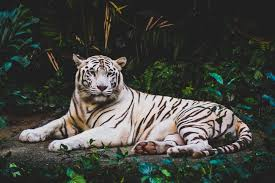
\includegraphics{index.jpeg}
\caption{LOGO}
\end{figure}
\subsection{Latex}



Document in Latex Document in Latex Document in LatexDocument in Latex Document in LatexDocument in Latex Document in Latex Document in LatexDocument in Latex Document in LatexDocument in LatexDocument in Latex.Document in Latex.Document in Latex.Document in Latex Document 
in LatexDocument in Latex Document in Latex Document in LatexDocument in Latex Document in 
LatexDocument in Latex Document in Latex Document in LatexDocument in Latex Document in LatexDocument 
\begin{figure}[H]
\centering
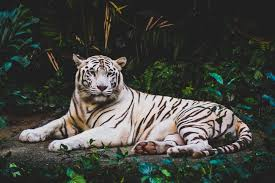
\includegraphics{index.jpeg}
\caption{LOGO}
\end{figure}
\subsection{Latex}

in LatexDocument in Latex.Document in Latex.Document in Latex.Document in Latex Document in LatexDocument in Latex Document in Latex Document in LatexDocument in Latex Document in LatexDocument in Latex Document in Latex Document in LatexDocument in Latex Document in LatexDocument in LatexDocument in Latex.Document in Latex.Document in Latex.Document in Latex Document in LatexDocument in Latex Document in Latex Document in LatexDocument in Latex Document in LatexDocument in Latex Document in Latex Document in LatexDocument in Latex Document in LatexDocument in Latex



\begin{center}

\begin{tabular}{|c|c|c|c|}
\hline
name & age & gender & course   \\
\hline
Anu & 19	& Female & BCA \\
\hline
Rahul & 20 & Male & BBA\\
\hline
\end{tabular}

\end{center}

\section{Listing}
\begin{itemize}
\item one

\begin{enumerate}[label=\Alph*]
\item first
\item second
\item third
\item fourth
\end{enumerate}

\item two
\item three
\item four
\end{itemize}


\section{Conclusion} Created for demonstration purpose only.
\chapter{Latex commands}
\section{Content 1} Prepared on \textit{\textbf{January 10th}}.
Prepared on january 10th 2020.\\Prepared as in image  \ref{fig1} .\\ Prepared on january 10th 2020.Prepared on january 10th 2020.Prepared on january 10th 2020.Prepared on january 10th 2020.Prepared on january 10th 2020.Prepared on january 10th 2020.Prepared on january 10th 2020.
\section{Content 2} Prepared on \textit{\textbf{January 10th}}.
\begin{figure}[h!]
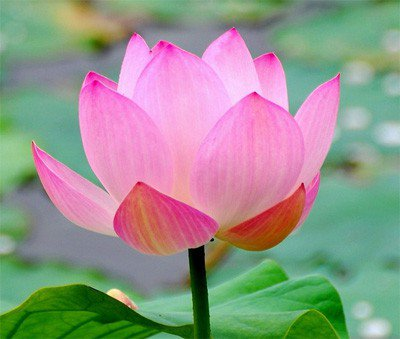
\includegraphics[scale=0.25]{Summer_Flowers_Lotus.jpg}
\caption{img}
\label{fig1}
\end{figure}

Prepared on january 10th 2020.Prepared on january 10th 2020.Prepared on january 10th 2020.Prepared on january 10th 2020.Prepared on january 10th 2020.Prepared on january 10th 2020.Prepared on january 10th 2020.Prepared on january 10th 2020.Prepared on january 10th 2020.



\section{Conclusion} Created for demonstration purpose only.
\end{multicols}
 
\textbf {this file need to be edited ...............}
\end{document}